\chapter{Spectroscopic Sky Surveys}
\label{data_chapter}

We start with a brief introduction to astronomical spectroscopy to understand the data used in this thesis.
Then, we describe quasars because they are the object we would like to identify in the Large Sky Area Multi-Object Spectroscopic Telescope survey using the data and labels from the Sloan Digital Sky Survey.
Therefore, we introduce the two large spectroscopic surveys in the following section.
We end this chapter with a comparison of the two surveys to show
that they are different, thus suitable for the problem of domain adaptation.

\section{Astronomical Spectroscopy}

Almost all we know about the universe outside our solar system is based on the analysis of light.
For example, we observe its flux or time variations.~\cite{appenzeller2012}.
Light is \textit{electromagnetic} (EM) radiation.
Spectroscopy started when Issac Newton experimented with light decomposition through a prism in 1666.
Next, Thomas Young has shown that light behaves like a wave.
However, EM radiation exhibits also particle nature.

The particles of EM radiation are photons.
Photons have no mass but transport energy and have momentum.
Every photon has an associated frequency \(\nu\) of the corresponding EM wave
giving it energy by the Planck--Einstein relation:

\begin{equation}
	E = h \nu,
	\label{planck_einstein_equation}
\end{equation}

where \(h\) is the Planck constant and \(\nu\) is the frequency of the photon.
Therefore, a higher frequency means higher energy.
All photons in vacuum move in the speed of light \(c\).
The frequency \(\nu\) is related to the wavelength \(\lambda\):

\begin{equation}
	\nu = \frac{c}{\lambda},
	\label{frequency_wavelength_equation}
\end{equation}

where \(c\) is the speed of light.
Combining equations~\ref{planck_einstein_equation} and \ref{frequency_wavelength_equation} gives:

\begin{equation}
	E = h \frac{c}{\lambda}.
	\label{energy_wavelength}
\end{equation}

We see that the energy of a photon is inversely proportional to wavelength \(\lambda\).~\cite{trypsteen2017}

Secondly, EM radiation has the wave nature. 
EM wave also propagates in the speed of light \(c\) and transfers energy.
Again the higher the frequency, the more energy it carries.~\cite{cochard2018}

EM wave can be decomposed (by a prism or a diffraction grating) as a function of its wavelength \(\lambda\).
The complete decomposed spectrum of EM radiation is called the EM spectrum.
The visible light is only a tiny part of the complete spectrum of electromagnetic radiation.
The complete spectrum consists of \(\gamma\)~rays, X-rays, ultraviolet, visible light, infrared radiation, microwaves, radio waves (see Table~\ref{em_spectrum}).

\begin{table}
\begin{center}
\begin{tabular}{|l|r|}
	\hline
	Radiation type & Wavelength (m) \\ \hline \hline
	\(\gamma\) ray & \(10^{-12}\) \\ \hline
	X-ray & \(10^{-10}\) \\ \hline
	Ultraviolet & \(10^{-8}\) \\ \hline
	Visible & \(0.5 \times 10^{-6}\) \\ \hline
	Infrared & \(10^{-5}\) \\ \hline
	Microwave & \(10^{-2}\) \\ \hline
	Radio & \(10^{3}\) \\ \hline
\end{tabular}
\end{center}
\caption{Parts of electromagnetic spectrum}
\label{em_spectrum}
\end{table}

Firstly, EM radiation is produced by either heating up matter or by exciting atoms.
The blackbody is a physical model of spectral radiation \(B(\lambda, T)\).
Max Planck derived the spectral distribution of a black body.
Heating transforms into emission of EM radiation at all wavelengths
with an energy distribution as a function of a wavelength
which only depends on the temperature and is described by Planck's law:

\begin{equation}
	B(\lambda, T) = \frac{2 h c^2}{\lambda^5}
	\frac{1}{e^{\frac{hc}{\lambda k_{\mathrm{B}}T}} - 1},
\end{equation}

where \(k_{\mathrm{B}}\) is the Boltzmann constant 
and \(h\) is the Planck constant.
This phenomenon does not depend on the composition of the body
but only on its temperature.
The Wien's displacement law gives the wavelength of maximum intensity \(\lambda_{\max}\):

\begin{equation}
	\lambda_{\max} = \frac{b}{T},
\end{equation}

where \(b\) is the Wien's displacement constant.
Accordingly, we can derive the temperature \(T\) of an object
with known wavelength of maximum intesity \(\lambda_{\max}\):

\begin{equation}
	T = \frac{b}{\lambda_{\max}},
\end{equation}

where \(b\) is the Wien's displacement constant.~\cite{cochard2018}

We consider stars to be black bodies
because they are objects hotter than its environment
and emit electromagnetic radiation.
Therefore, all EM radiation of a star is determined only by its temperature.
The other way around, with the Wien's displacement law,
we can estimate the absolute temperature \(T\) of a star.~\cite{trypsteen2017}

Secondly, EM radiation can be emitted by exciting atoms.
Therefore, EM radiation carries information about stars and planets
made of matter across the universe.
The energy carried by EM radiation interacts with matter in the following ways:

\begin{itemize}
	\item \textit{emission} occurs when EM radiation propagates through a gas
		because the atoms of the gas might excite and emit EM radiation;
	\item \textit{absorption} happens when a gas absorbs some wavelengths
		of the EM radiation.
\end{itemize}

Fraunhofer was also one of the first to observe dark lines in the solar spectrum
and David Brewster postulated that the dark lines correspond to absorption from gas in the way of light travelling towards us.
Robert Wilhelm Bunsen and Gustav Kirchhoff showed that each chemical element has its own set of spectral lines
and Kirchhoff established the three famous laws describing the three types of spectra:

\begin{itemize}
	\item the spectrum of a conventional light bulb is a continuous rainbow (called \textit{continuous spectrum});
	\item if a cloud of gas lies between a detector and a bulb,
		the cloud can absorb specific wavelength making what an \textit{absorption-line spectrum};
	\item if a cloud emits light itself, its spectrum is called an \textit{emission-line spectrum}.
\end{itemize}

Real astronomical spectra are usually a combination of these types.
Therefore, spectroscopy can be used for chemical analysis of the matter.
Then, at the beginning of the twentieth century,
the invention of quantum mechanics help us to understand the origin of spectral lines.

We model matter as made of atoms.
An atom has a specific number of electrons which are place in particular orbits of the atom.
Electrons in an orbit have a specific energy level.
We know from quantum mechanics that an electron can change energy level by an exchange of energy in the form of a photon.
The energy transfer is not continuous.
The energy has to correspond to the difference in the energy levels precisely.
Therefore, the change produces EM radiation with an energy \(E\) in the wavelength \(\lambda\)
according to Planck--Einstein relation in~Equation~\ref{energy_wavelength}.
Therefore, the specific set of energy levels of an atom determines
if photons are either absorbed or emitted by it,
which is a direct consequence for spectroscopy.~\cite{cochard2018}

The fact that each atom, ion or molecule possesses a unique set of energy levels
causes emission and absorption lines at specific wavelengths in spectra.
Spectral lines correspond to the wavelengths of light absorbed by chemicals on the surface of the star.
Therefore, positions of emission and absorption lines can tell us objects composition.
We display spectra as bands of light that is a projection of light
that passes through a prism on a wall (see Figure~\ref{solar_spectrum})
called \textit{two-dimensional} spectra.~\cite{cochard2018}

\begin{figure}
% source https://solarsystem.nasa.gov/resources/390/the-solar-spectrum/
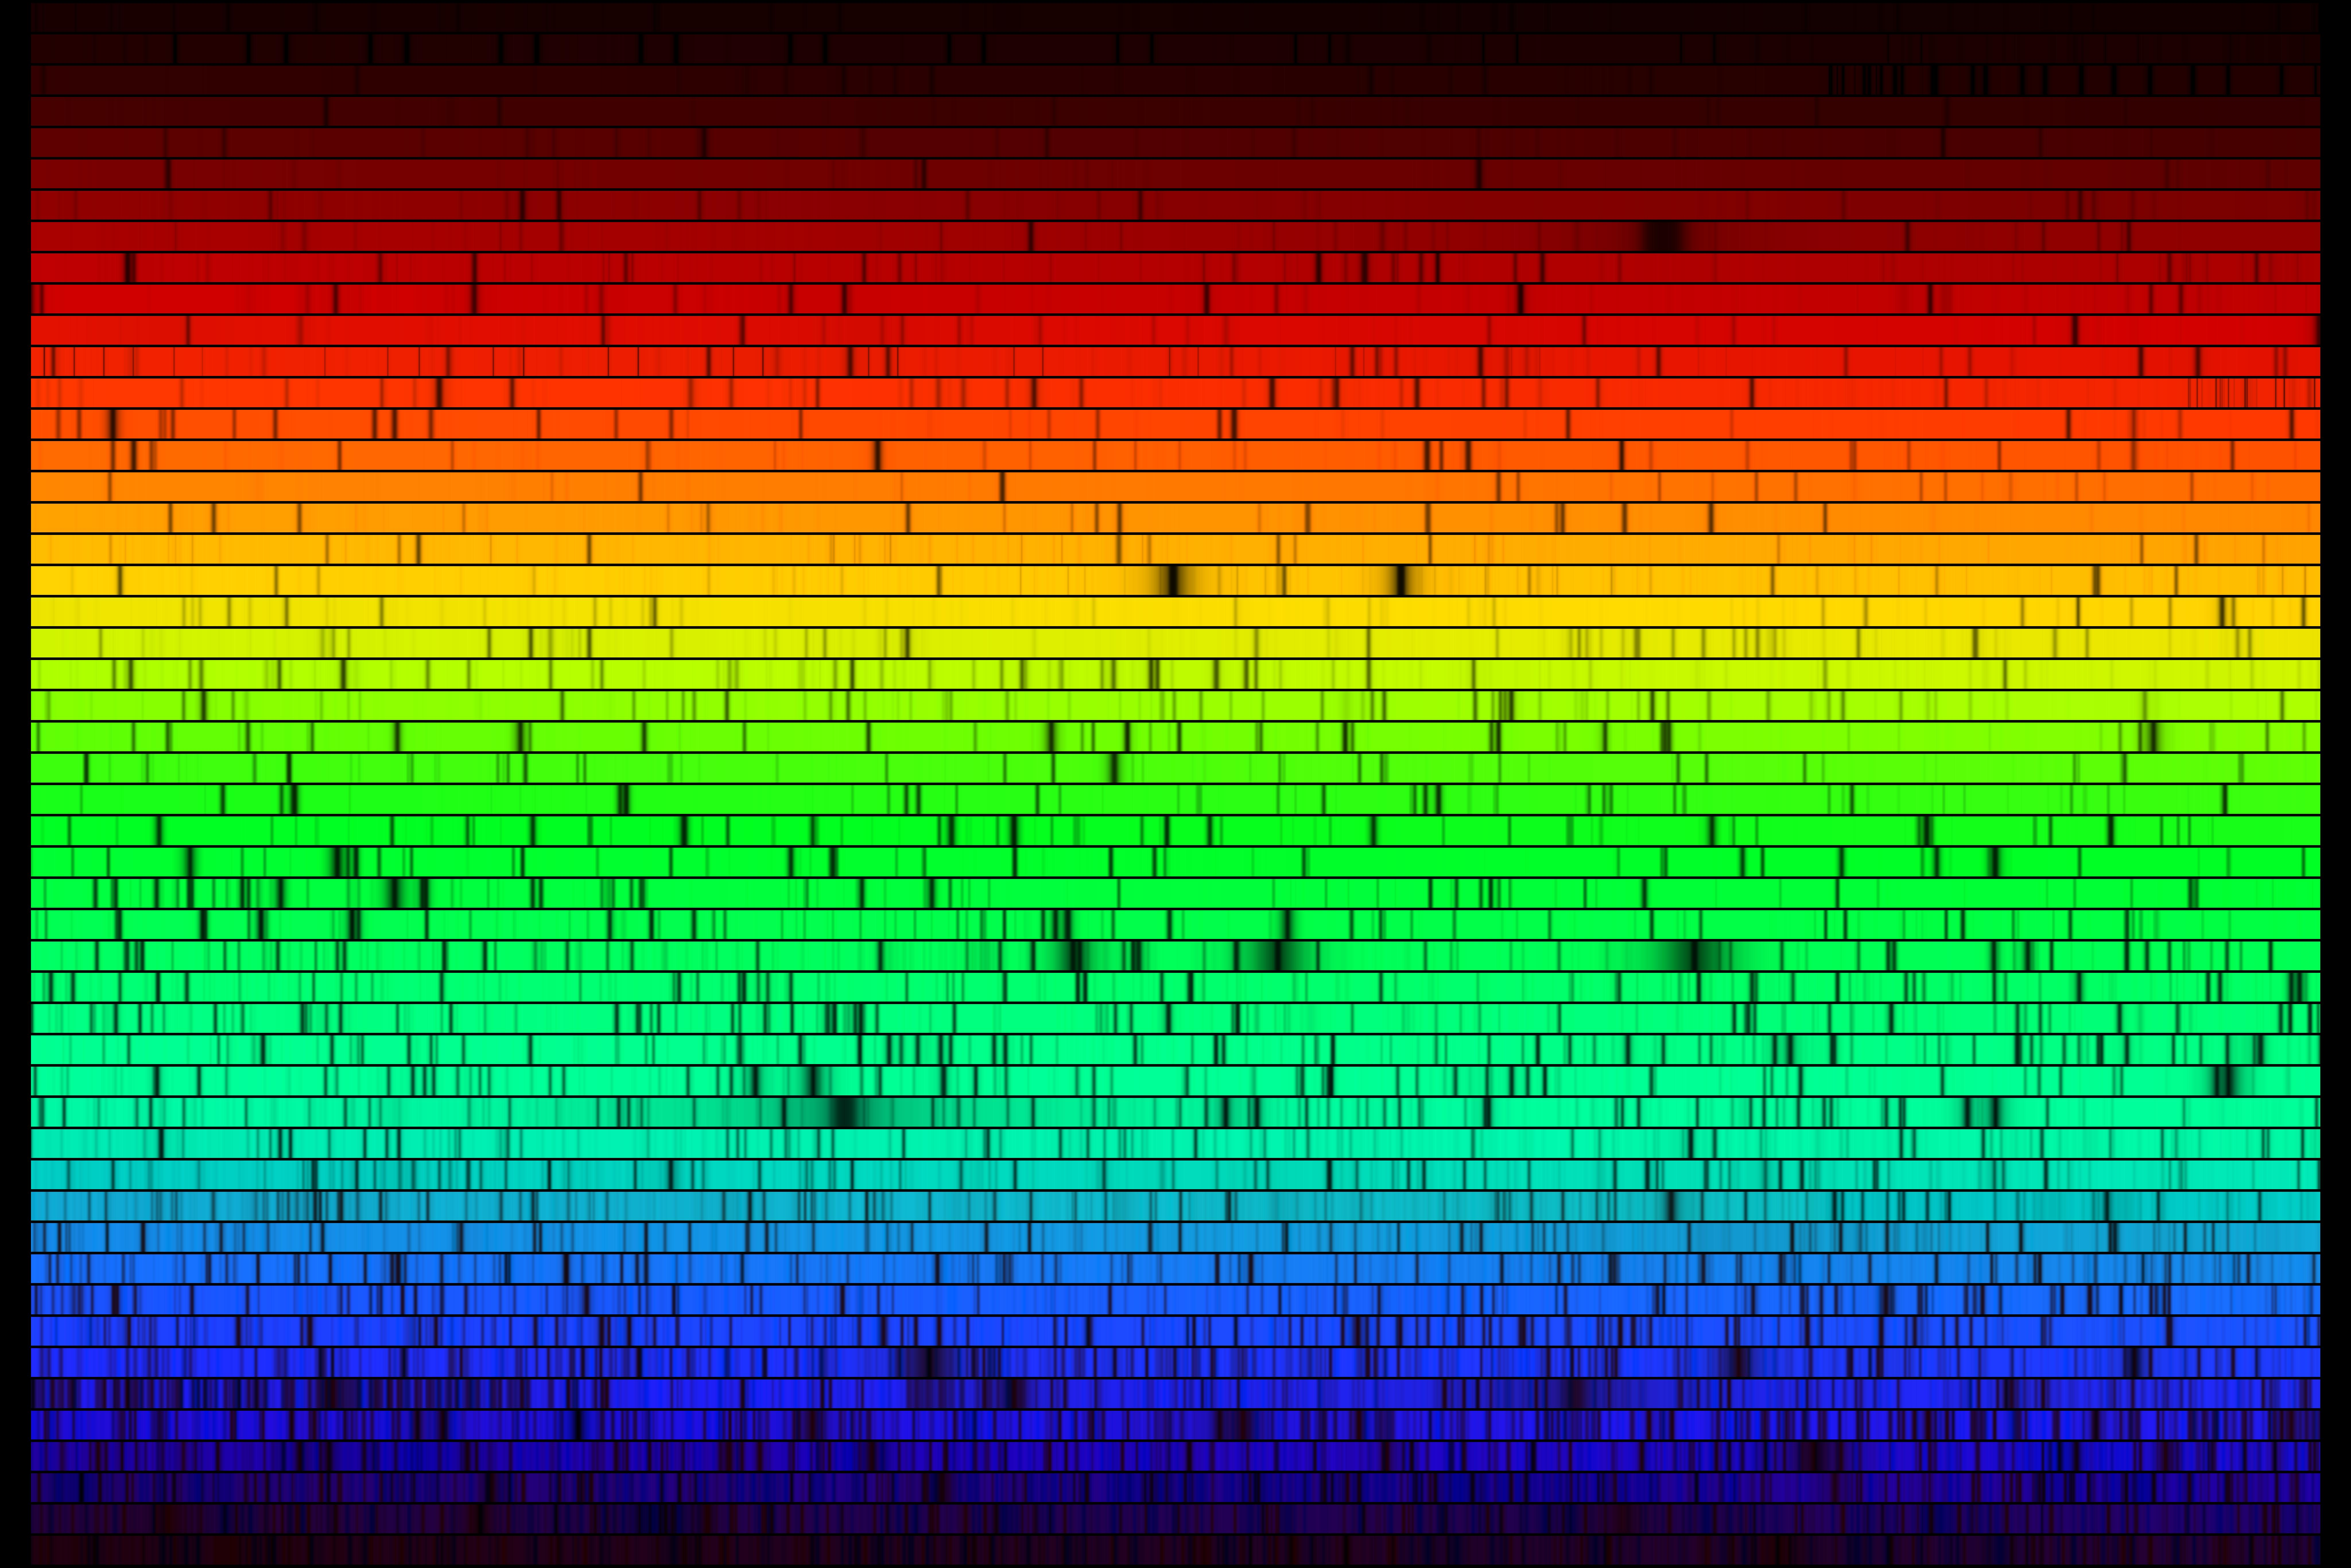
\includegraphics[width=\textwidth]{img/solarspectrum.jpg}
\caption[Two-dimensional Solar spectrum]{
	The two-dimensional specturm of the Sun by \href{https://solarsystem.nasa.gov/resources/390/the-solar-spectrum/}{NASA}.
}
\label{solar_spectrum}
\end{figure}

A more reasonable way is to display spectra as graphs of intensities of the light as the vertical axis and wavelengths as the horizontal axis:
called a \textit{one-dimensional spectral profile}
(see Figure~\ref{3c_273_spectrum}).~\cite{cochard2018, bennett2005}
This representation of an astronomical spectrum can be seen as a one-dimensional image.

\begin{figure}
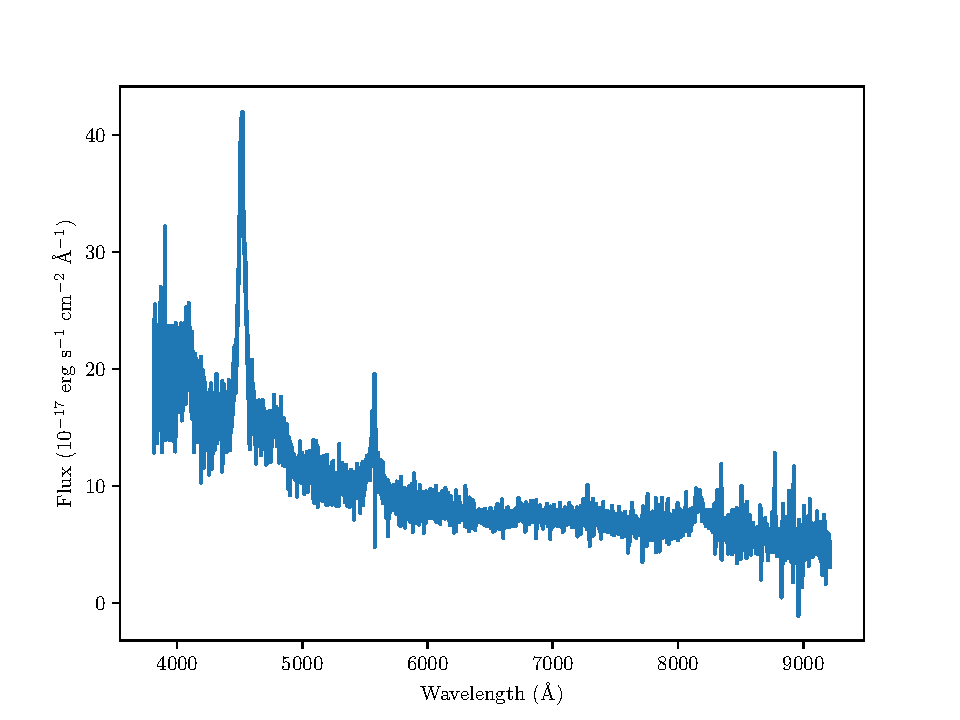
\includegraphics[width=\textwidth]{img/spec_3c_273.pdf}
\caption[One-dimensional spectum of the quasar 3C 273]{
	The one-dimensional spectral profile of the first ever discovered quasar 3C 273.
}
\label{3c_273_spectrum}
\end{figure}


Joseph von Fraunhofer was the first to observe spectra of stars by using a spectroscope in combination with a telescope.
Nowadays, new technologies have advanced spectroscopic observations
(CCD detectors, optical fibres and computing power).~\cite{cochard2018}
Telescopes are giant eyes than can collect much more light that the eye of a human.
A telescope is composed of mirrors and lenses that lead light into a spectrograph.
A spectrograph contains a diffraction grating and a \textit{charge-coupled device} (CCD) camera.
Fraunhofer invented diffreaction grating based on the wave nature of light.
It can disperse the light collected by a telescope into a spectrum
while allowing more excellent dispersion than prisms.
Diffraction gratings are one of the essential parts of modern spectroscopes.
Then, the dispersed spectrum reveals objects composition, speed, temperature
and more.~\cite{bennett2005}

Photons carry information about observed objects
to a pixel of a CCD camera in a telescope.
CCD cameras require the particle nature of light (electromagnetic radiation).~\cite{trypsteen2017}

An important parameter of a telescope is its \textit{field of view}
and important parameters of a spectrograph are \textit{spectral resolving power}, \textit{signal-to-noise ration} and \textit{full width at half maximum} for our purposes.

Spectral resolving power \(R\) expresses the capacity of a telescope to observe details of a spectrum
and is defined as:

\begin{equation}
	R = \frac{\lambda}{\Delta \lambda},
\end{equation}

where \(\lambda\) is considered wavelength
and \(\Delta \lambda\) is the smallest visible detail.
Signal-to-noise ratio (SNR) determines how much we can trust our measurement
concenring the power of the signal in comparison to noise.
Full width at half maximum (FWHM) is the measurement of the width of a spectral line at the half of its maximum intensity measured from the continuum.
FWHM is determined by the width of a slit which makes the broadening of a line.
A perfect instrument would have an infinitely thin line.~\cite{cochard2018}

\section{Quasi-Stellar Objects}

Quasi-stellar (star-like) objects (also known as \textit{quasars} and abbreviated \textit{QSO}) are the most luminous \textit{active galactic nuclei} (AGN).~\cite{beckmann2013}

The physical model is a supermassive black hole surrounded by a gaseous accretion disk and jets (see Figure~\ref{3c_273}).
A QSO generates energy by stress and friction in the disk outside of the black hole because no light can escape the \textit{event horizon}.
The energy is in the form of EM radiation is the strongest in the ultraviolet band.
Moreover, QSOs exhibit significat cosmological redshift.

\begin{figure}
\begin{center}
\subfloat[
	Image of the bright quasar 3C 273 by \href{https://www.spacetelescope.org/images/potw1346a/}{ESA/Hubble} is licensed under CC BY 4.0.
]{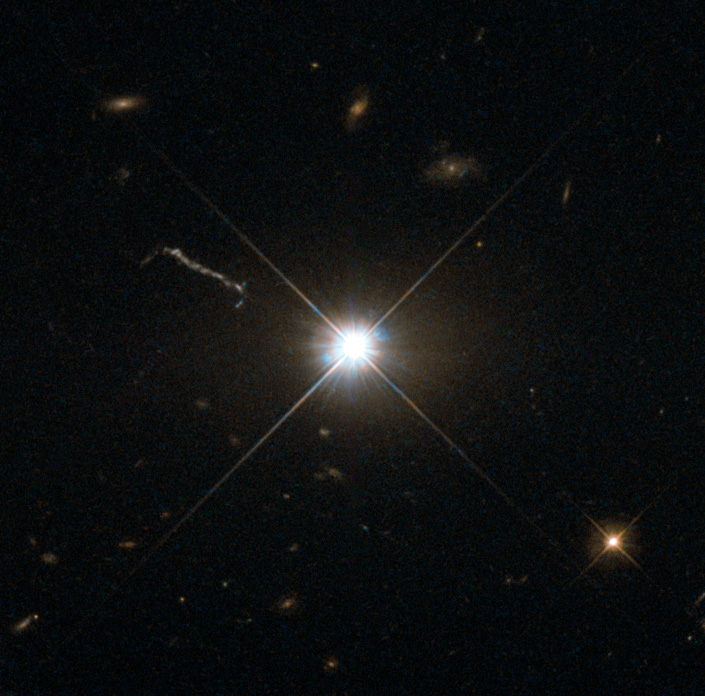
\includegraphics[height=0.45\textwidth]{img/potw1346a.jpg}}
\quad
\subfloat[
	Jet of the quasar 3C 273 by \href{https://chandra.harvard.edu/photo/2000/0131/index.html}{NASA/CXC/SAO/H. Marshall et al.}
]{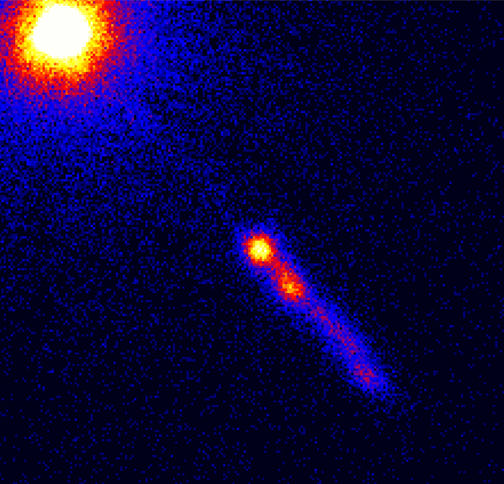
\includegraphics[height=0.45\textwidth]{img/0131_xray.jpg}}
\end{center}
\caption[Image and jet of the quasar 3C 273]{
	The left image demonstrate the star-like apperant of the QSO 273
	while the right image by the Chanda X-ray Obsevatory shows important details in the powerful jet shooting from the quasar 3C 273.
}
\label{3c_273}
\end{figure}

QSOs were common in the early universe probably because galaxies have run out of matter: they stop to be lumionous.
Therefore, QSOs help us to study the early universe.

There are different types of QSOs: radio-loud, radio-quiet, broad absorption-line, type II, red, optically violent variable, weak emission-line.

A typical spectrum of a QSO is redshifted and
contains a characteristical combination of broad and narrow emission lines.
A spectrum of a QSO from SDSS is shown in Figure~\ref{3c_273_spectrum}.

\section{Large Spectroscopic Surveys}
\label{large_spec_surveys}

Since the discovery of the first QSO,
there has been massive progress in spectroscopy,
allowing observing a vast amount of spectra and QSOs.
It started with the Bright Quasar Survey, Large Bright Quasar Survey (LBQS) and 2dF Quasar Redshift Survey.
Their significant successors are the \textit{Sloan Digital Sky Survey} (SDSS)
and the \textit{Large Sky Area Multi-Object Fiber Spectroscopic Telescope} (LAMOST)
that already contain millions of spectra.
We choose LAMOST and SDSS surveys for our experiments
because they offer a large volume of data suitable for machine learning
and for training neural networks for domain adaptation.

In the two following subsections,
we introduce the parameters of their instruments,
their recent data releases and corresponding catalogues of QSOs.

\subsection{Sloan Digital Sky Survey}
\label{sdss}

SDSS is in operation since 2000,
and its telescope is designed to provide both a photometrically
and astrometrically calibrated imaging survey
and a spectroscopic survey of galaxies and QSOs.~\cite{york2000}

The SDSS survey uses a 2.5~m telescope located at the Apache Point Observatory, New Mexico (see~Figure~\ref{sdss_telescope}).
The telescope has 3\(^{\circ}\) field of view due to its mirror.
The original spectrograph of the telescope was able to obtain 640 spectra
with a wavelength coverage 380--920~nm simultaneously
with spectral resolution \(R \sim 1\,800\).~\cite{york2000, gunn1998}

\begin{figure}
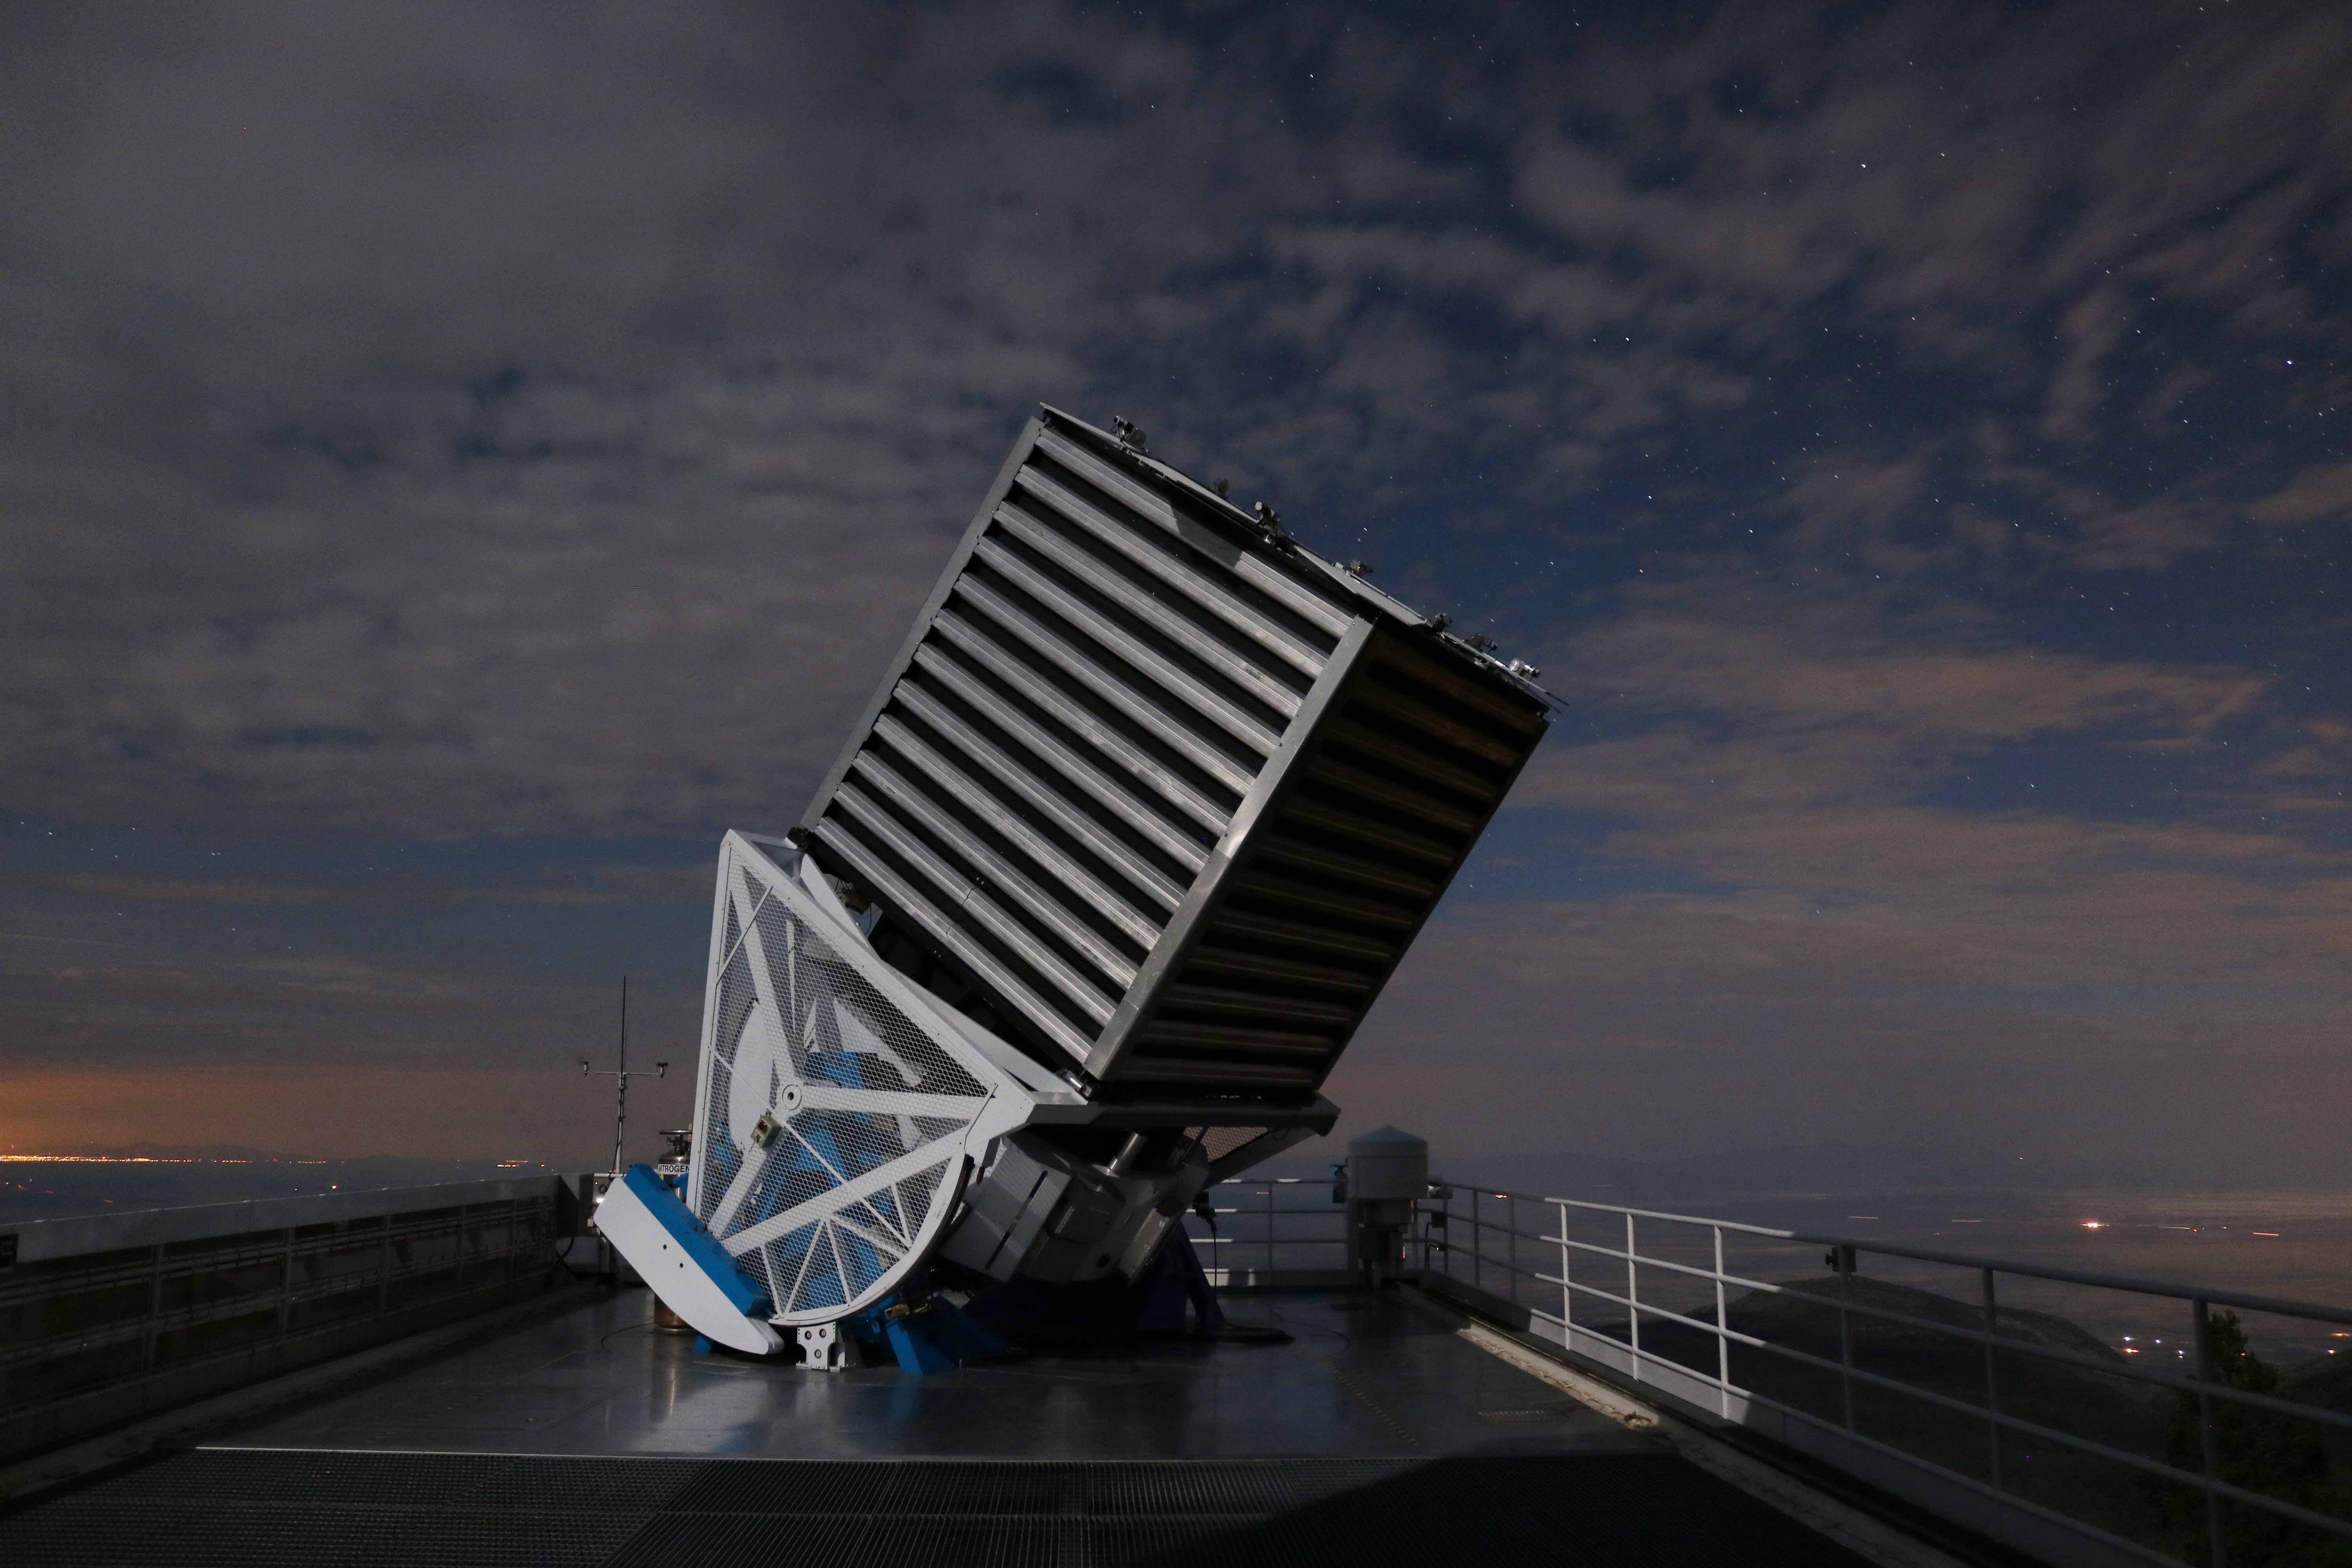
\includegraphics[width=\textwidth]{img/sdss_gaulme.jpg}
\caption[SDSS telescope]{
	The SDSS telescope at night located in the Apache Point Observatory, New Mexico, by \href{https://www.sdss.org/wp-content/uploads/2016/07/sdss_gaulme1.jpg}{Patrick Gaulme} is licensed under CC BY 4.0.
	}
\label{sdss_telescope}
\end{figure}

In 2009, the original spectrograph was upgraded for \textit{Baryon Oscillation Spectroscopic Survey} (BOSS).
The upgraded BOSS spectrograph covers a wavelength range 356--1\,040~nm
with resolving power \(R \sim 2\,000\)
and is capable to observe 1\,000 spectra at once.~\cite{smee2013}

Recent SDSS Data Release 14 (SDSS DR14) which corresponds to the latest catalogue of QSOs,
contains more than one-third of the entire celestial sphere.
The total number of optical spectra in the catalogue is 4\,851\,200.

The SDSS Data Release 14 Quasar (SDSS DR14Q) catalogue described in~\cite{paris2018} contains 526\,356 quasars
(contamination is estimated to be about 0.5\%).
SDSS provides calibrated spectra covering the wavelength range 3\,610--10\,140~\AA{} at a spectral resolution 1\,300 < \(R\) < 2\,500 for all the QSOs.

The catalogue defines a QSO as an object with a certain luminosity in a specific distance
and either displaying at least one emission line with FWHM > 500~km~s\(^{-1}\)
or having interesting absorption features.

\subsection{Large Sky Area Multi-Object Fiber Spectroscopic Telescope}
\label{lamost}

LAMOST survey was launched in 2012.
Its two primary scientific goals are to explore both extragalactic and intragalactic phenomenons.
Therefore, unlike SDSS, LAMOST also observes a large volume of stars.
However, the other scientific goal of LAMOST is the extragalactic spectroscopic survey of the large scale structure of the universe and the physics of galaxies.
The goal includes a spectroscopic survey of nearly 10 million galaxies and \textit{quasars}
that will contribute to the study of the accretion process of massive black holes in AGNs besides other things.~\cite{cui2012}

The LAMOST is located in Xinglong Station of National Astronomical Observatory, China.
The telescope is a special telescope with a primary mirror made of 37 hexagonal spherical mirrors of total size 6.67~m times 6.05~m.
The large primary mirror makes a field of view of 5\(^{\circ}\).
The focal surface has 4\,000 fibres connected to 16 spectrographs with 32 CCD cameras.
Therefore, the telescope is capable of observing up to 4\,000 spectra simultaneously
in wavelength coverage of 370--900~nm with spectral resolution \(R = 1\,000\) or \(R = 1\,500\) depending on gratings and camera positions.~\cite{cui2012}

LAMOST Data Release 5 v3 (LAMOST DR5) is the lastest data release
which has corresponding catalogue of QSOs.
The LAMOST DR5 contains 9\,026\,365 optical spectra,
and the catalogues of QSOs of interest are DR1~\cite{ai2016}, DR2\&3~\cite{dong2018} and DR4\&5~\cite{yao2019}
that in total contains 42\,552 spectra of QSOs.

\subsection{Comparison of the Spectral Data}
\label{comparison}

Now, we compare the SDSS and LAMOST survey to prove their suitability for domain adaptation.
The surveys are mainly different in term of instruments, sky coverage and targeting strategy.

We summarise the main parameters of instruments of the surveys in Table~\ref{telescopes_parameters}.
We see that LAMOST has lower resolution and shorter wavelength coverage than SDSS.
However, SDSS has a smaller field of view.

\begin{table}
\begin{center}
\begin{tabular}{|l|r|r|r|}
	\hline
	Parameter of an instrument & SDSS & BOSS & LAMOST \\
	\hline \hline
	Wavelength coverage (nm) & 380--920 & 356--1\,040 & 370--900 \\
	\hline
	Spectral resolution \(R\) & 1\,800 & 2\,000 & 1\,250 \\
	\hline
	Field of view & 3\(^{\circ}\) & 3\(^{\circ}\) & 5\(^{\circ}\) \\
	\hline
\end{tabular}
\end{center}
\caption[Parameters of the LAMOST and SDSS instruments]{
	We list the parameters of the LAMOST and SDSS instruments
	to compare their different parameters.
	The instrument of SDSS has higher spectral resolution and wider wavelength coverages
	while LAMOST can observer bigger areas of the sky.
	}
\label{telescopes_parameters}
\end{table}

Sky coverage is very connected to the targeting strategy or scientific goals.
Figure~\ref{sky_coverage} displays sky coverage of both SDSS and LAMOST.
We see that SDSS does not observe our Milky Way galaxy.
On the other hand, LAMOST observes everywhere on the northern hemisphere
but is not able to observe close to zenith due to its construction limits.
From the perspective of coverage of QSOs depicted in Figure~\ref{qso_coverage},
LAMOST did not observe QSOs in some part of the sky where QSOs are abundant according to SDSS.

\begin{figure}
\subfloat[
	Sky coverage of SDSS corresponds to its primary scientific goal to observe galaxies and QSOs.
	Therefore, it has almost no observations in the area of our Milky Way galaxy.
]{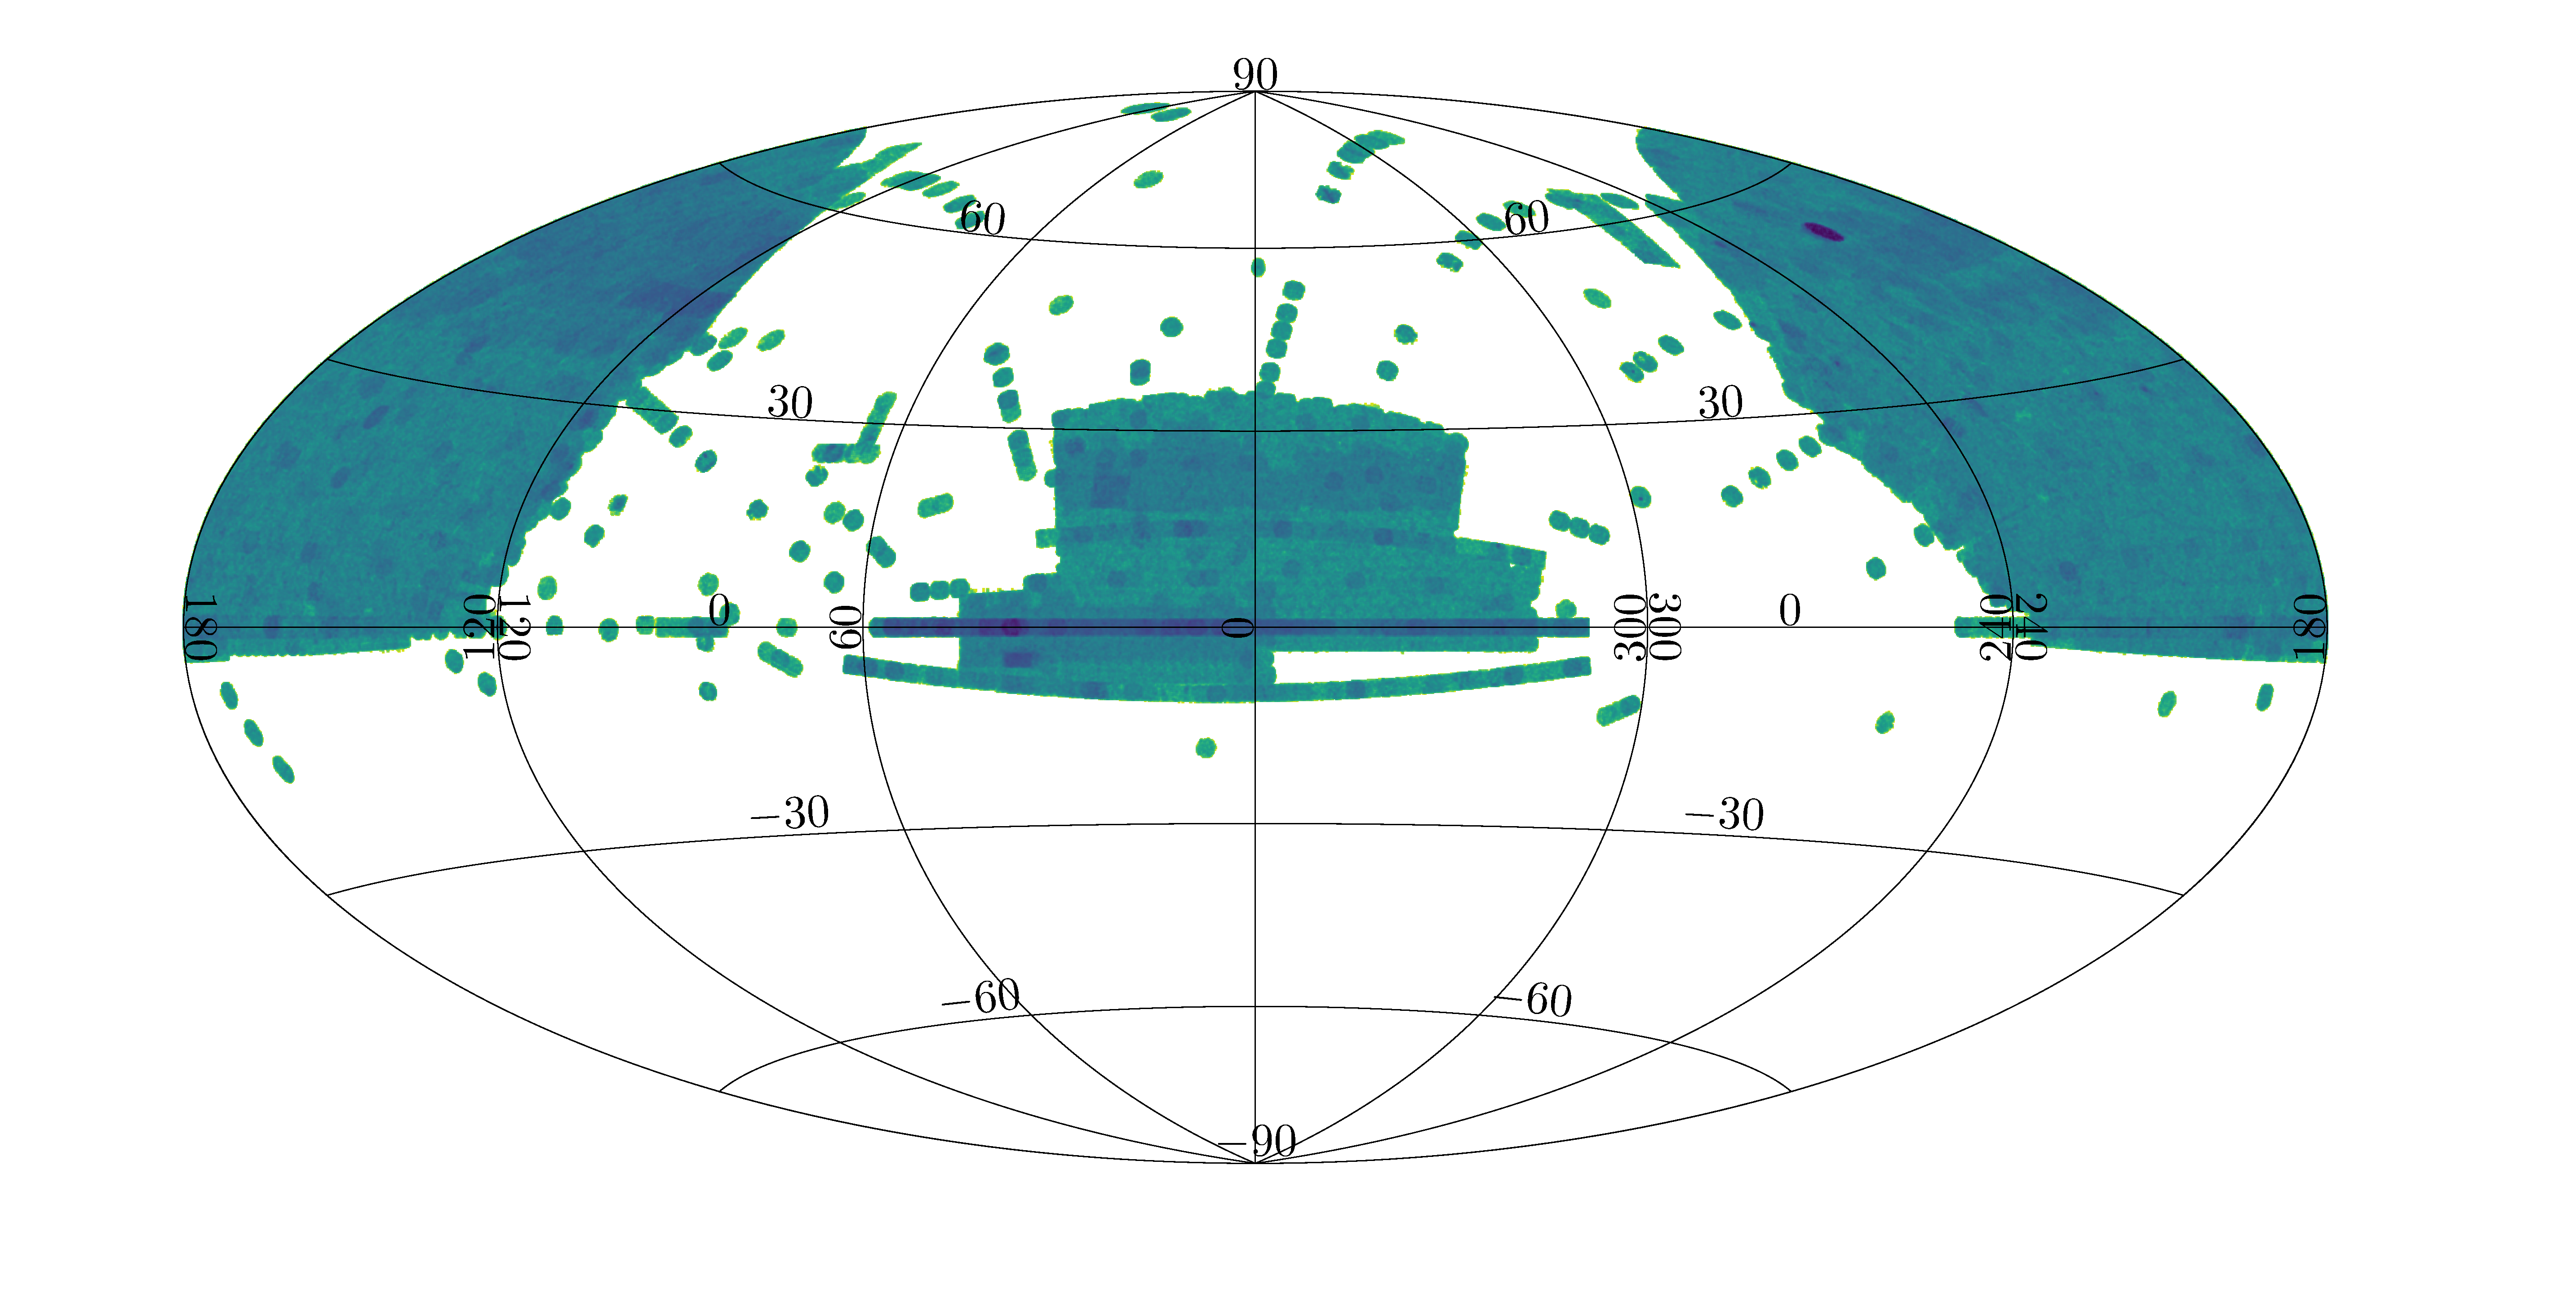
\includegraphics[width=\textwidth]{img/sdss.pdf}}\\
\subfloat[
	LAMOST observes both the extragalactic and intragalactic objects.
	Therefore, its distribution of observation almost uniform on the northern hemisphere.
	An exception is the surroundings of zeniths due to the telescope construction limits.
]{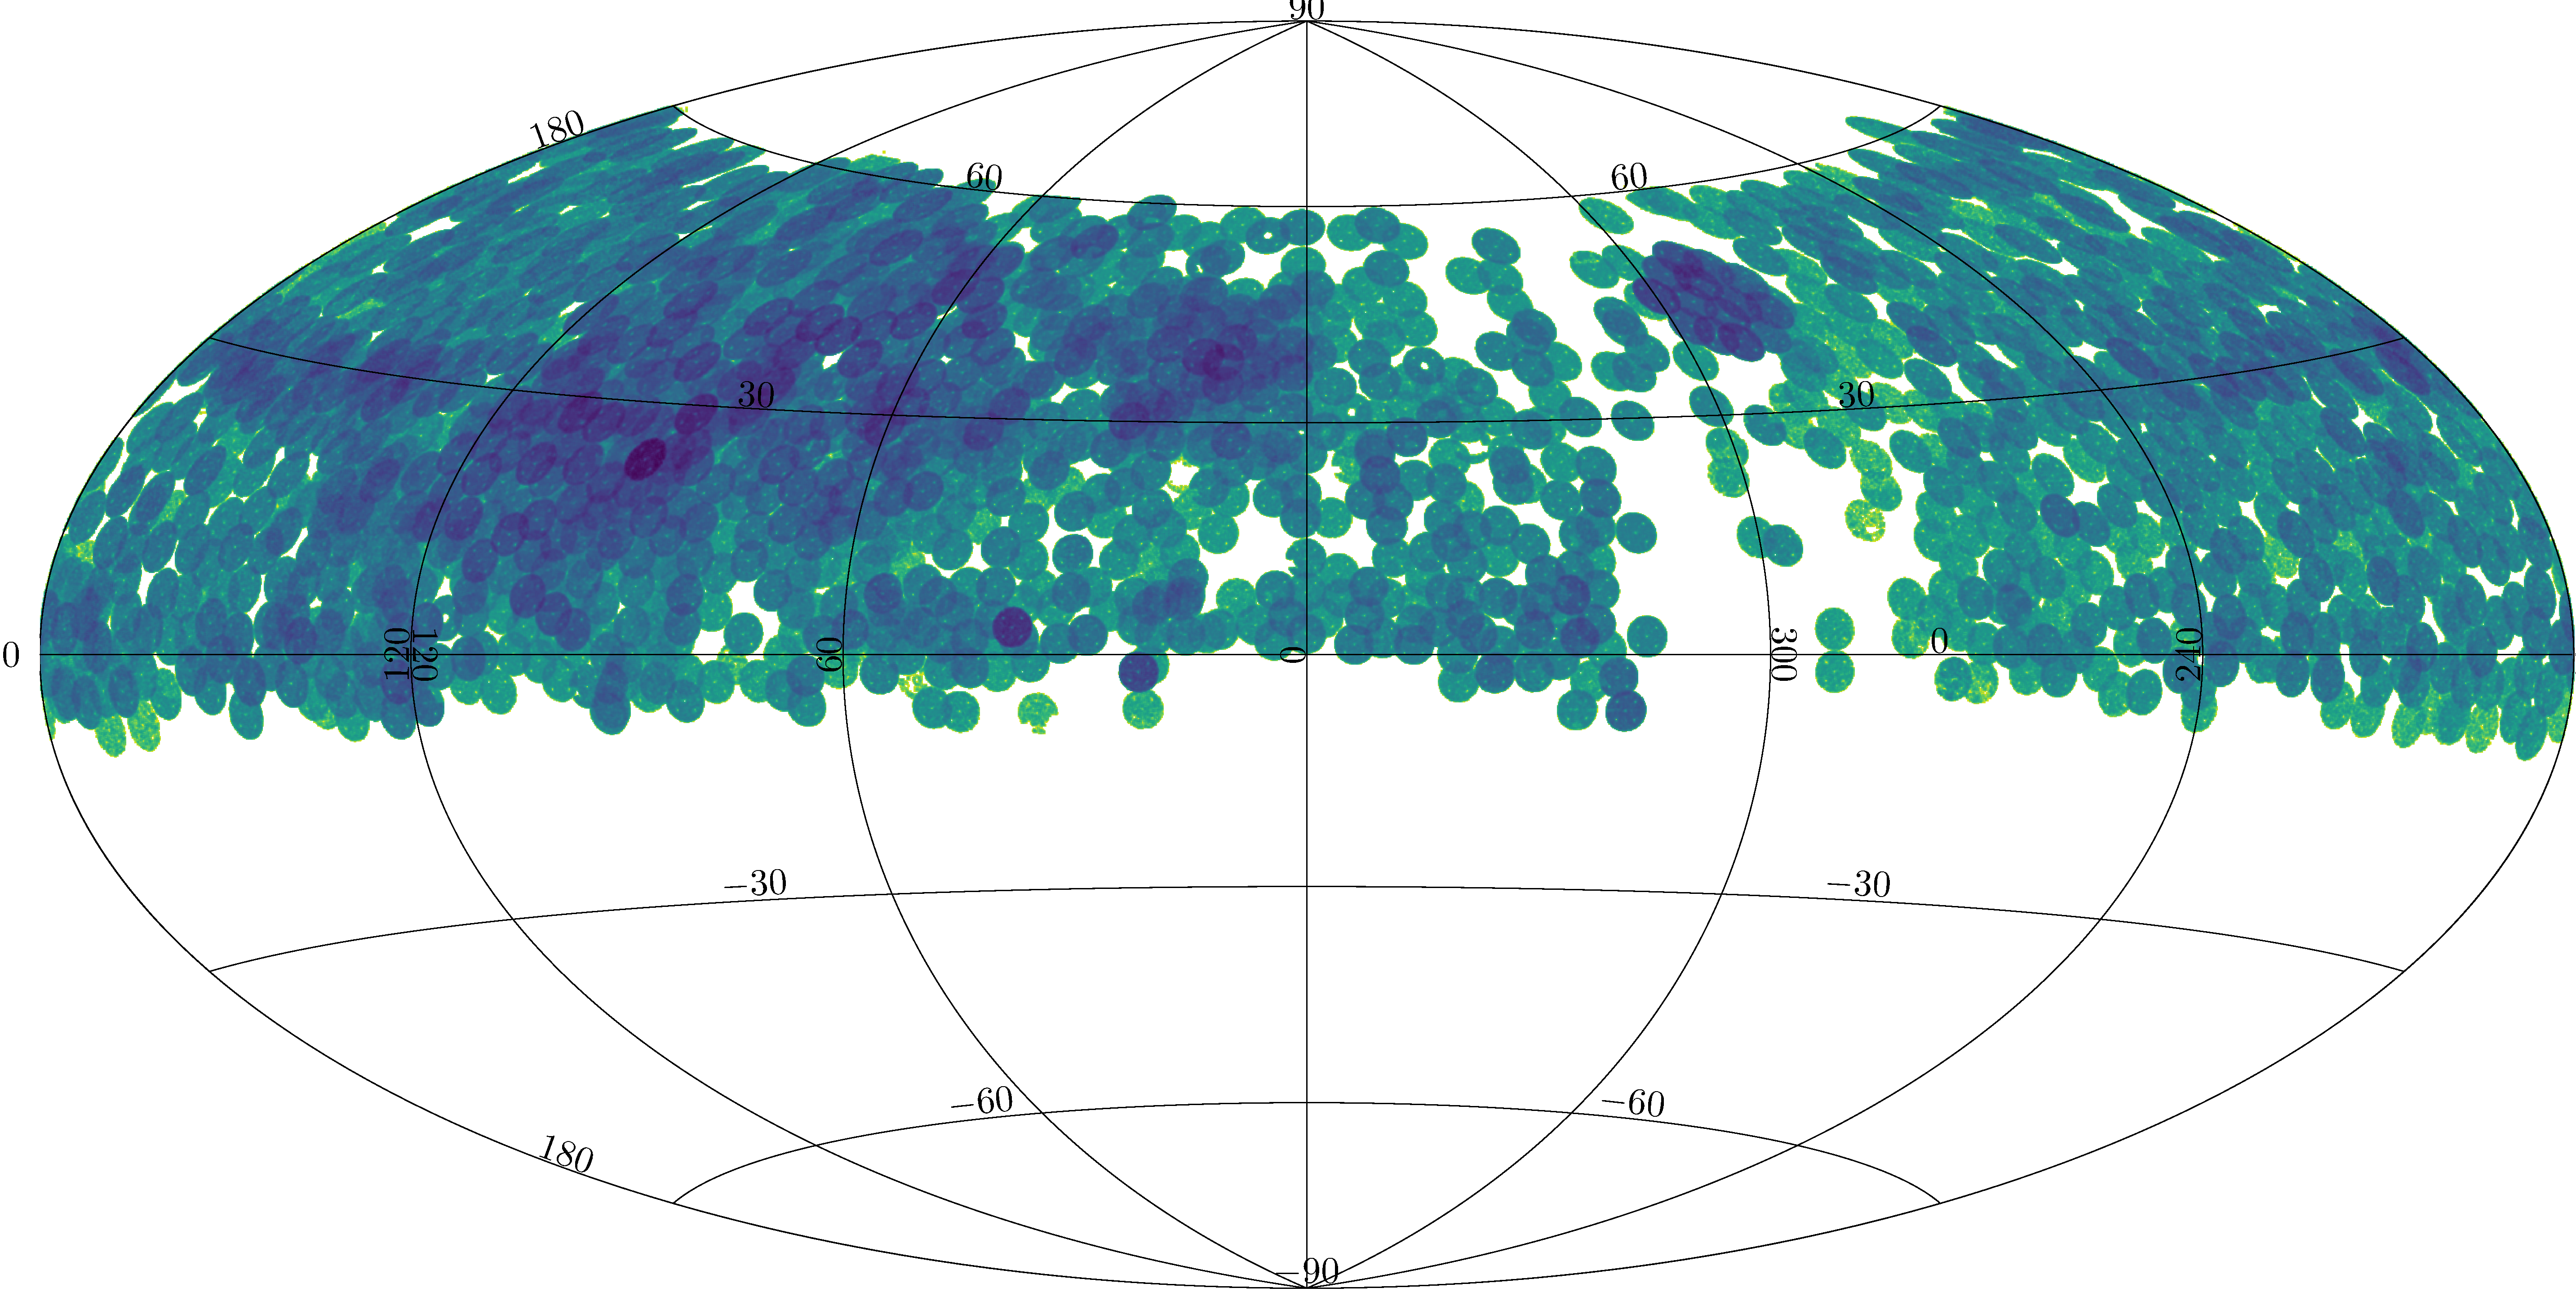
\includegraphics[width=\textwidth]{img/lamost.pdf}}
\caption[Sky coverage of SDSS and LAMOST]{
	Comparison of sky coverage of SDSS and LAMOST.
}
\label{sky_coverage}
\end{figure}

\begin{figure}
\subfloat[
	SDSS can identify quasars everywhere it has observations.
]{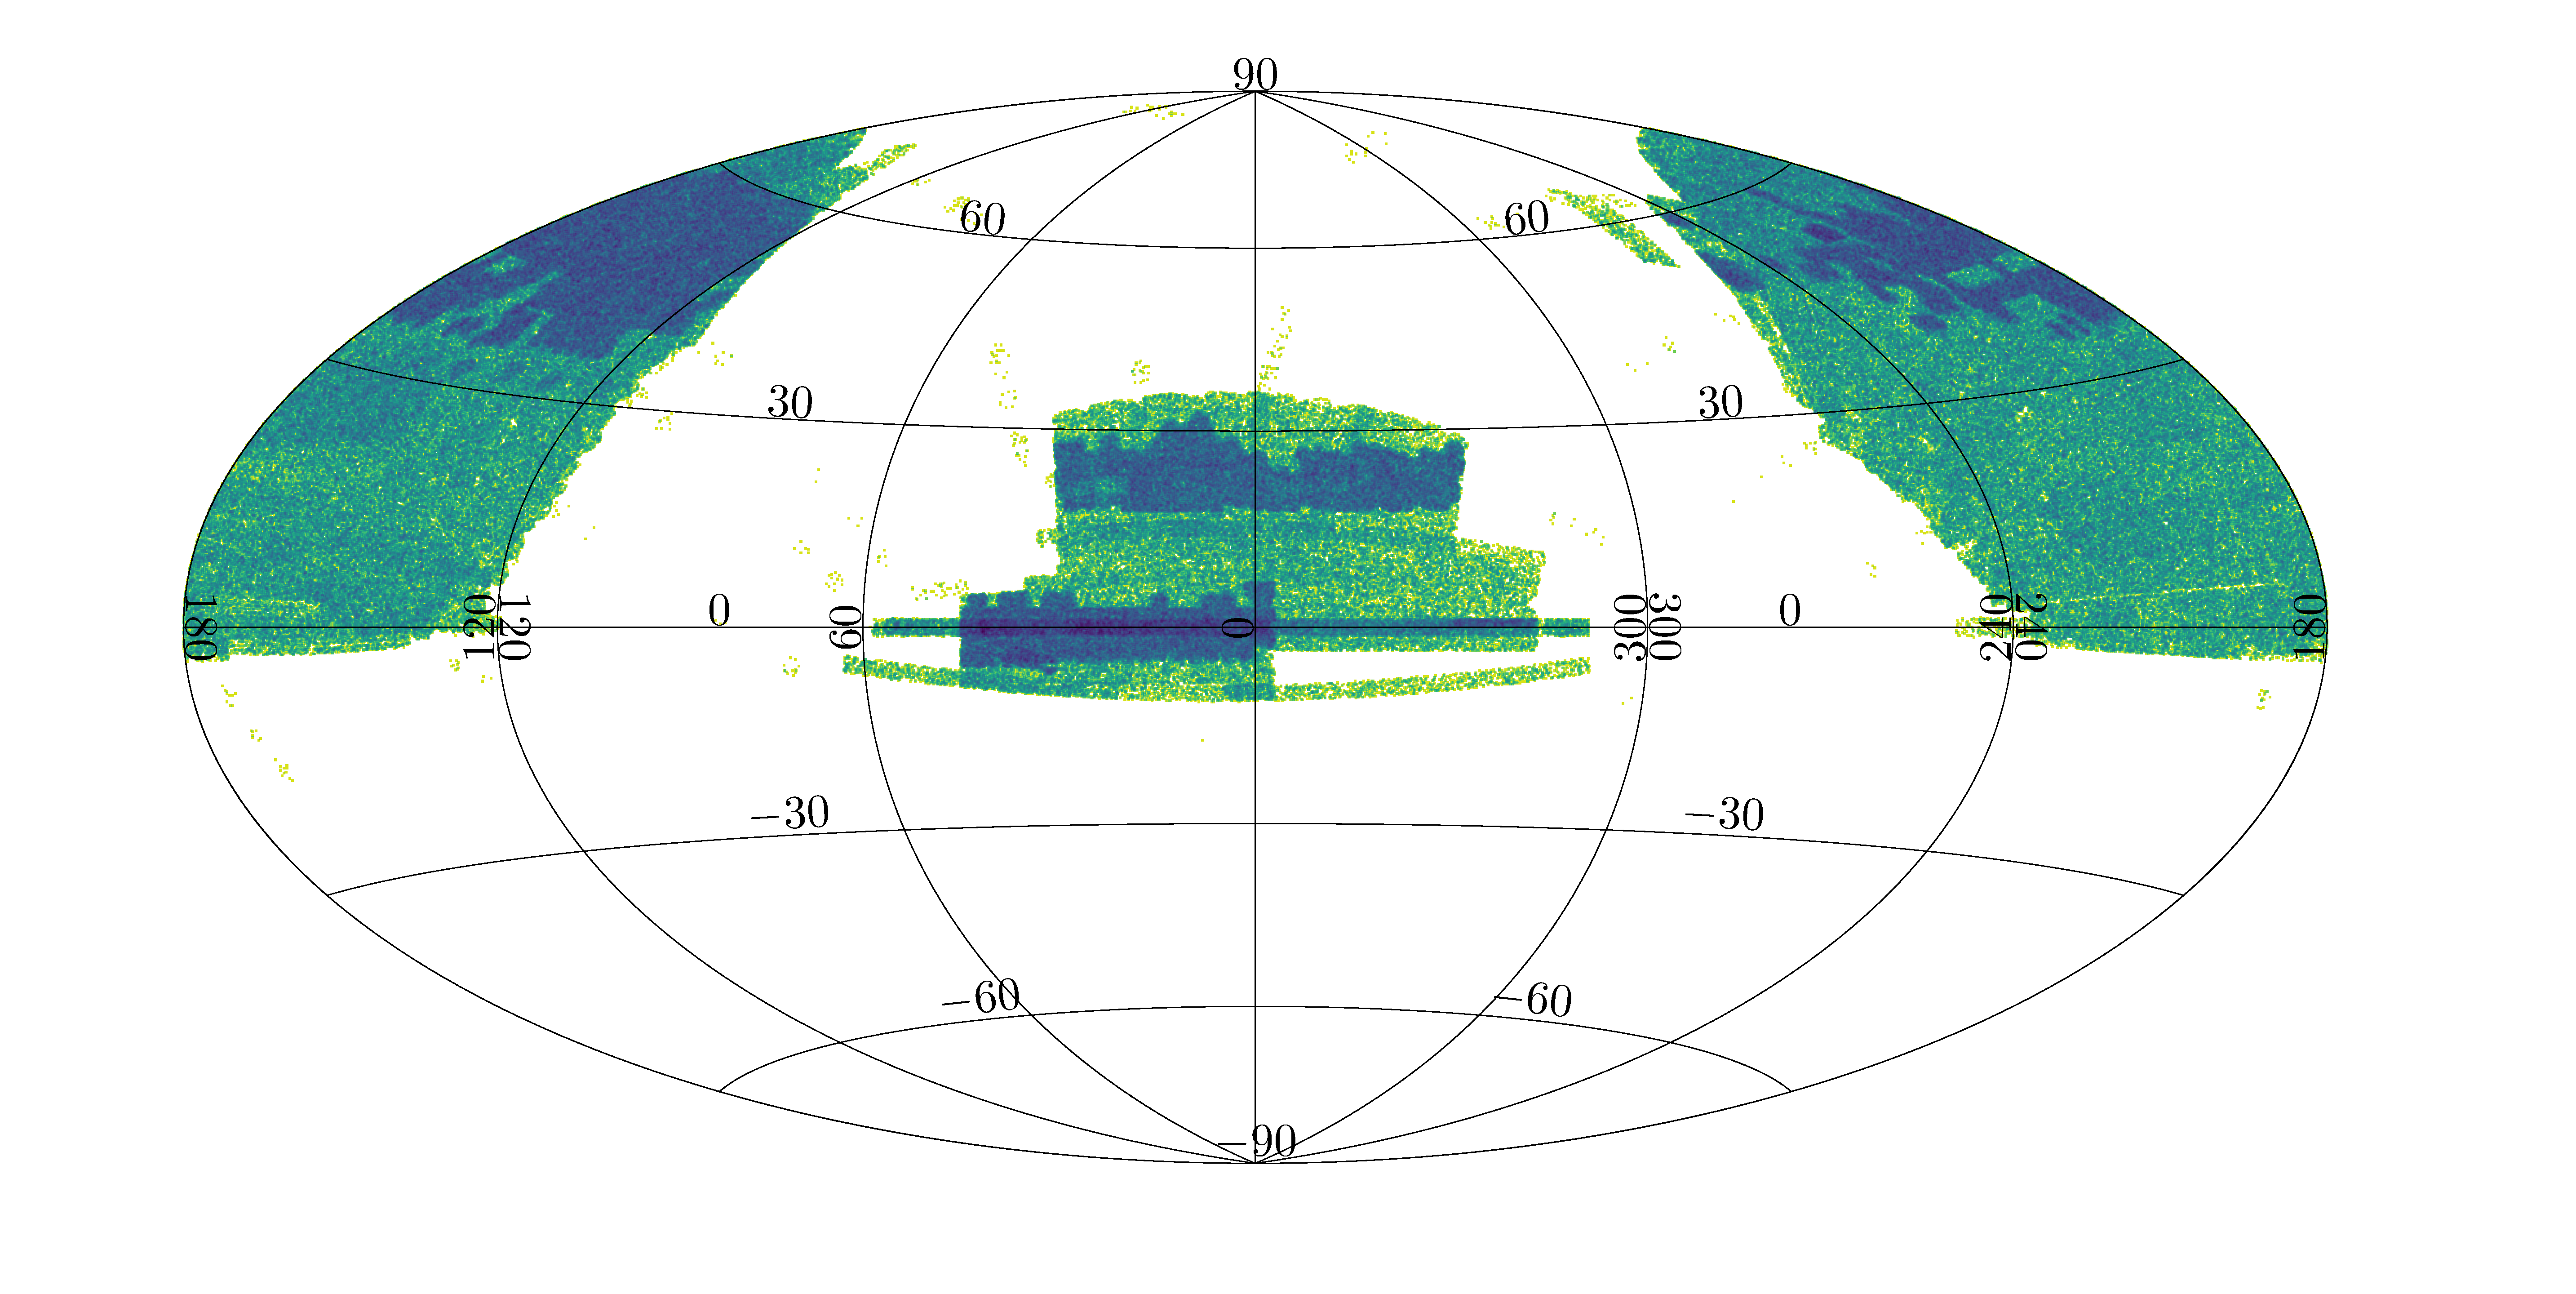
\includegraphics[width=\textwidth]{img/sdss_qso.pdf}}\\
\subfloat[
	Although LAMOST has observations in similar areas as SDSS,
	its catalogues contain only small amount of QSOs in comparison to SDSS.
]{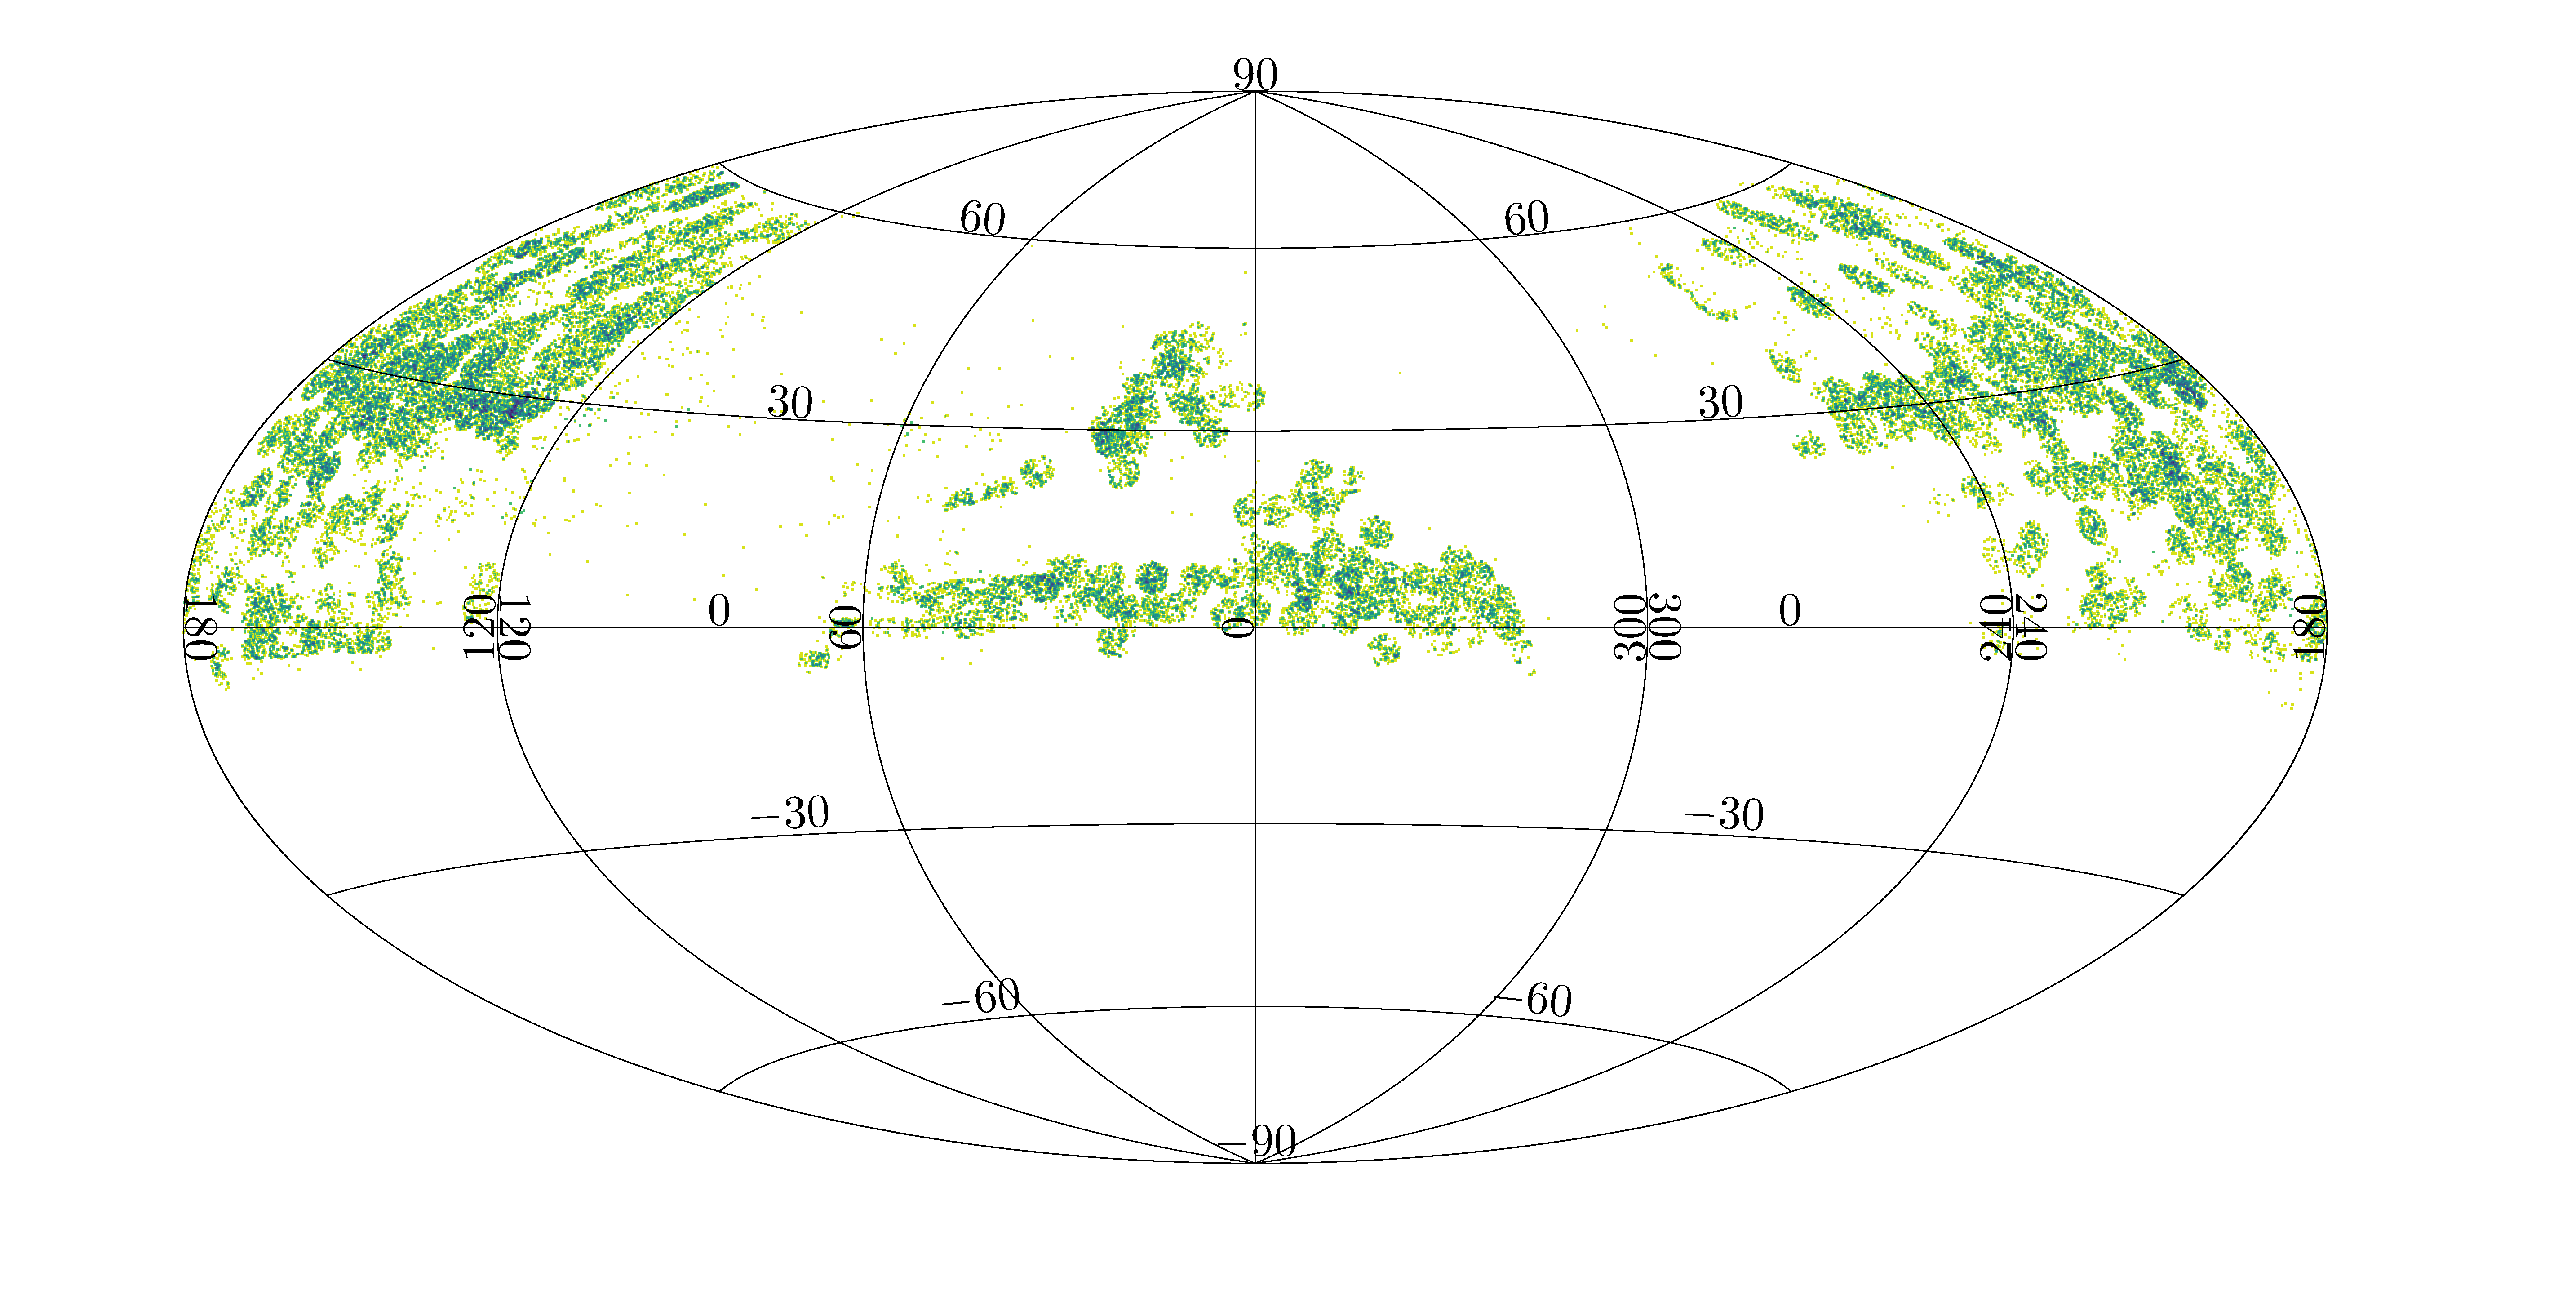
\includegraphics[width=\textwidth]{img/lamost_qso.pdf}}
\caption[Sky position of quasars of SDSS and LAMOST]{
	Sky positions of QSOs listed in either SDSS or LAMOST catalogues.
}
\label{qso_coverage}
\end{figure}

We conclude that the two surveys seem to be suitable for domain adaptation
because their instruments create spectra with different resolution and wavelength range.
Moreover, observations of SDSS and LAMOST survey has different distributions.
